\newpage
\section{Recurrent Neural Networks}
Process Sequences

\begin{figure}[!htb]
    \centering
    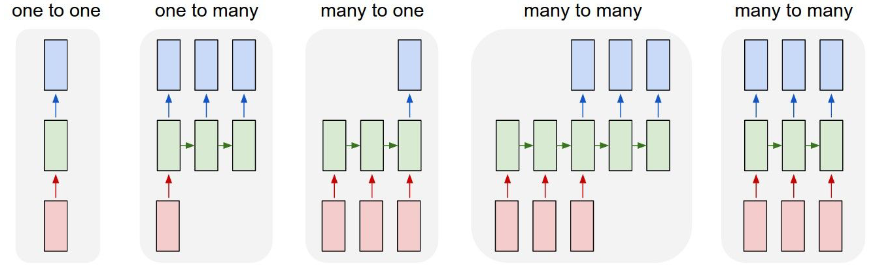
\includegraphics[width=0.42\textwidth]{pic/Lec10/Process Sequences.png}
    \caption{Process Sequences}
\end{figure}

Sequential Processing of Non-Sequence Data, e.g. Classify images by taking a series of ``glimpses''. 

RNN process a sequence of vectors x by applying a recurrence formula at every time step:
\begin{align*}
    h_t=f_W(h_{t-1}, x_t)
\end{align*}

\begin{itemize}
    \item $h_t$: new state
    \item $h_{t-1}$: old state
    \item $f_W$: some functions with parameters $W$
    \item $x_t$: input vector at some time step 
\end{itemize}

% \begin{figure}[!htb]
%     \centering
%     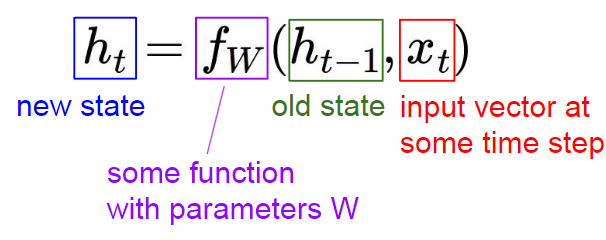
\includegraphics[width=0.309\textwidth]{pic/Lec10/RNN.png}
%     % \caption{RNN}
% \end{figure}

将在每个时间重复使用 $f_W$ 及 $W$. 

\subsection{(Vanilla) Recurrent Neural Network}
The state consists of a single ``hidden'' vector $\mathbf{h}$: 
\begin{align*}
    h_t&=f_W(h_{t-1}, x_t)\\
    & \downarrow\\
    h_t&=\tanh (W_{hh}h_{t-1}+W_{xh}x_t)\\
    y_t&=W_{hy}h_t
\end{align*}

\begin{figure}[!htb]
    \centering
    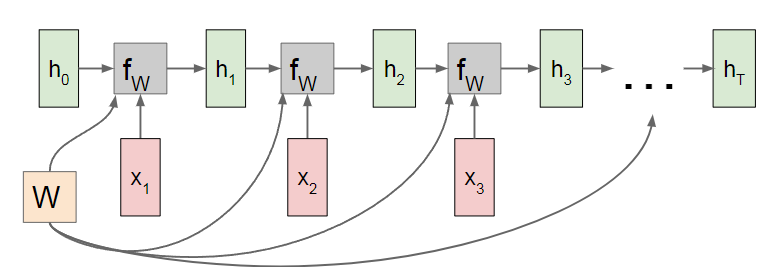
\includegraphics[width=0.42\textwidth]{pic/Lec10/RNN Computational Graph}
    \caption{RNN Computational Graph}
\end{figure}

e.g. Character-level Language Model Sampling

\begin{figure}[!htb]
    \centering
    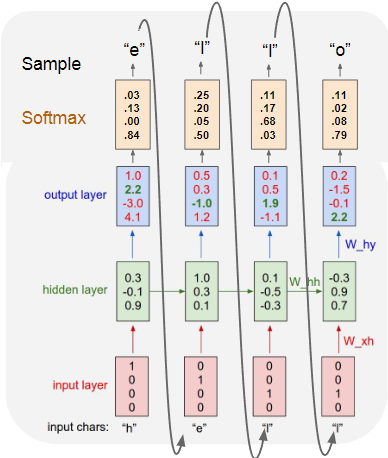
\includegraphics[width=0.42\textwidth]{pic/Lec10/Character-level Language Model Sampling}
    \caption{Character-level Language Model Sampling}
\end{figure}

\subsubsection{Backpropagation through time}
Backpropagation through time: 在整个序列中前向传播计算 loss, 然后反向传播计算损失. (每次要过全部的训练数据, 难以接受)

\textbf{Truncated} Backpropagation through time: 一块块序列进行 forward 与 backward. 具体的, 维护 forward 的隐藏层, 然后仅 backward 几层. 

e.g. From 教科书的 latex or linux source generated 新的东西. 就是预测下一个字符. 

探索向量的作用: e.g. 管理引号的, 管理换行的, 在代码中管理 if 语句的, 缩进的. 

\subsection{Image Captioning}
输入: 图片的特征向量 (经过了例如 VGG的前几层)

输出: 总结图片内容的单词.

\subsubsection{Image Captioning with Attention}

\begin{figure}[!htb]
    \centering
    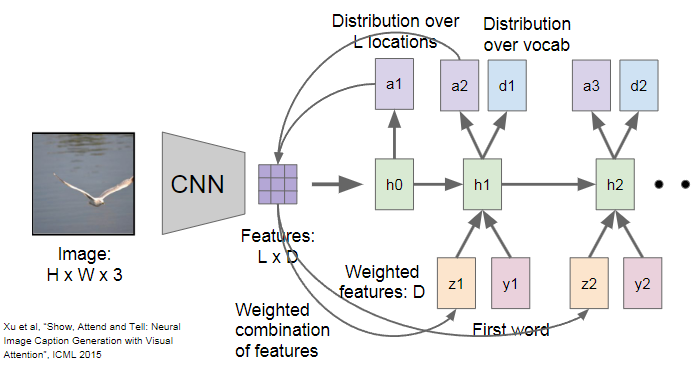
\includegraphics[width=0.42\textwidth]{pic/lec10/attention.png}
    \caption{attention}
\end{figure}

将图片的位置同样作为输入. 有 soft 和 hard 的区别, soft 是全局位置加权, hard 是强制选择一个位置. 

RNN 可以多层. 

\subsection{Vanilla RNN Gradient Flow}
Backpropagation from $h_t$ to $h_{t-1} $ multiplies by $W$ (actually by $W_{hh}^T$). 但这样 $h_0$ 的梯度会被所有 $W$ 影响, 基本要么爆炸, 要么消失.

\begin{align*}
    h_t&=\tanh(W_{hh}h_{t-1}+W_{xh}x_t)\\
    &=\tanh\left( \begin{pmatrix}
        W_{hh} & W_{xh}
    \end{pmatrix}\begin{pmatrix}
        h_{t-1} \\ x_t
    \end{pmatrix} \right)\\
    &=\tanh\left( W\begin{pmatrix}
        h_{t-1}\\ x_t
    \end{pmatrix} \right)
\end{align*}

\begin{figure}[!htb]
    \centering
    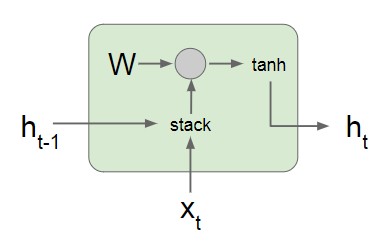
\includegraphics[width=0.309\textwidth]{pic/Lec10/Vanilla RNN}
    \caption{Vanilla RNN}
\end{figure}

爆炸梯度可使用 gradient clipping 解决, 但消失需要使用更复杂的RNN结构. 
\subsection{Long Short Term Memory (LSTM)}

\begin{align*}
    \begin{pmatrix}
        i\\f\\o\\g
    \end{pmatrix}&=\begin{pmatrix}
        \sigma \\ \sigma \\ \sigma \\ 
        tanh
    \end{pmatrix}W\begin{pmatrix}
        h_{t-1}\\x_t
    \end{pmatrix}\\
    c_t&=f\odot c_{t-1} + i\odot g\\
    h_t&=o\odot \tanh c_t
\end{align*}

$h_t$ 是传递的, $c_t$ 是本地的. 

\begin{figure}[!htb]
    \centering
    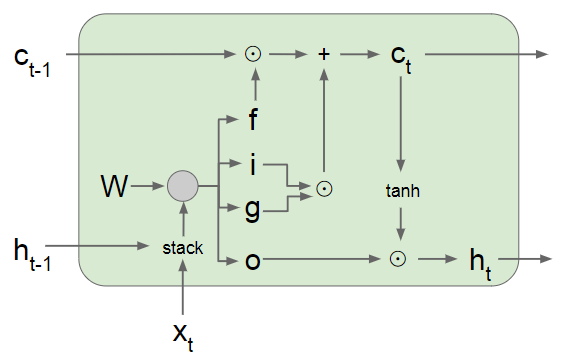
\includegraphics[width=0.309\textwidth]{pic/Lec10/LSTM.png}
    \caption{LSTM}
\end{figure}

\begin{itemize}
    \item $\mathbf{f}$: \textbf{Forget gate}, Whether to erase cell
    \item $\mathbf{i}$: \textbf{Input gate}, whether to write to cell
    \item $\mathbf{g}$: \textbf{Gate gate} (?), How much to write to cell
    \item $\mathbf{o}$: \textbf{Output gate}, How much to reveal cell    
\end{itemize}

Backpropagation from $c_t$ to $c_{t-1}$ only elementwise multiplication by $f$, no matrix multiply by $W$. 可以保证$c$一条线的梯度被快速回传. 

\subsection{Other RNN Variants}
e.g. GRU